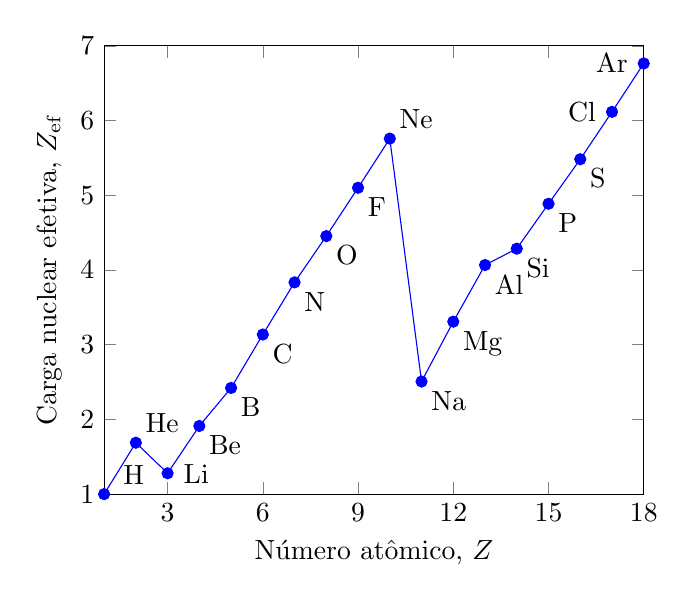
\begin{tikzpicture}
  \begin{axis}
    [
      grid = none,
      ylabel = {Carga nuclear efetiva, $Z_\mathrm{ef}$},
      xlabel = {Número atômico, $Z$},
      ymin=1, ymax=7,
      xmin=1, xmax=18,
      xtick = {0, 3, 6, 9, 12, 15, 18},
      ytick = {1, 2, 3, 4, 5, 6, 7},
    ]       
    \addplot [ mark=*, color=blue ] coordinates
      { 
        (01, 1.000)
        (02, 1.688)
        (03, 1.279)
        (04, 1.912)
        (05, 2.421)
        (06, 3.136)
        (07, 3.834)
        (08, 4.453)
        (09, 5.100)
        (10, 5.758)
        (11, 2.507)
        (12, 3.308)
        (13, 4.066)
        (14, 4.285)
        (15, 4.886)
        (16, 5.482)
        (17, 6.116)
        (18, 6.764)
      };
  
    \node [anchor = south west] at (axis cs:1.3, 1.000) { H  };
    \node [anchor = south west] at (axis cs:2, 1.688) { He };
    \node [anchor = west] at (axis cs:3.2, 1.27) { Li };
    \node [anchor = north west] at (axis cs:4, 1.912) { Be };
    \node [anchor = north west] at (axis cs:5, 2.421) { B  };
    \node [anchor = north west] at (axis cs:6, 3.136) { C  };
    \node [anchor = north west] at (axis cs:7, 3.834) { N  };
    \node [anchor = north west] at (axis cs:8, 4.453) { O  };
    \node [anchor = north west] at (axis cs:9, 5.100) { F  };
    \node [anchor = south west] at (axis cs:10, 5.758) { Ne };
    \node [anchor = north west] at (axis cs:11, 2.507) { Na };
    \node [anchor = north west] at (axis cs:12, 3.308) { Mg };
    \node [anchor = north west] at (axis cs:13, 4.066) { Al };
    \node [anchor = north west] at (axis cs:14, 4.285) { Si };
    \node [anchor = north west] at (axis cs:15, 4.886) { P  };
    \node [anchor = north west] at (axis cs:16, 5.482) { S  };
    \node [anchor = east] at (axis cs:16.8, 6.116) { Cl };
    \node [anchor = east] at (axis cs:17.8, 6.764) { Ar };
  \end{axis}
\end{tikzpicture}